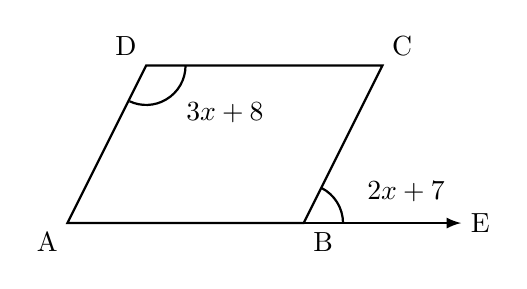
\begin{tikzpicture}[scale=1]

  % Define coordinates for the vertices of the parallelogram
  \coordinate (A) at (0,0);
  \coordinate (B) at (3,0);
  \coordinate (C) at (4,2);
  \coordinate (D) at (1,2);
  \coordinate (E) at (5,0);

  % Draw the parallelogram ABCD
  \draw[thick] (A) -- (B) -- (C) -- (D) -- cycle;

  % Draw the extended line from B to E with an arrow
  \draw[thick, ->, >=latex] (B) -- (E);

  % Add labels for the vertices
  \node[below left] at (A) {A};
  \node[below right] at (B) {B};
  \node[above right] at (C) {C};
  \node[above left] at (D) {D};
  \node[right] at (E) {E};

  % Draw arc for angle ADC (3x+8)
  % Angle is at D(1,2). Lines are DA and DC.
  % DA vector is (-1, -2). DC vector is (3, 0).
  % Let's just use simple arcs relative to D.
  \draw[thick] (1.5,2) arc (0:-115:0.5);
  \node at (2, 1.4) {$3x+8$};

  % Draw arc for angle CBE (2x+7)
  % Angle is at B(3,0). Lines are BC and BE.
  % BC vector is (1, 2). BE vector is (2, 0).
  \draw[thick] (3.5,0) arc (0:63.4:0.5);
  \node at (4.3, 0.4) {$2x+7$};

\end{tikzpicture}